\documentclass{colt2015}
\usepackage{amsmath}
\usepackage{caption}
\usepackage{amssymb}
\usepackage{amsfonts}
\usepackage{graphicx}

\newtheorem*{problem}{Open Problem}


\title{Open Problem: Learning Quantum Circuits with Queries}
\coltauthor{\Name{Jeremy Kun} \Email{jkun2@uic.edu}\\
\AND
\vskip -.25in
\noindent \Name{Lev Reyzin} \Email{lreyzin@math.uic.edu}\\
\addr Department of Mathematics, University of Illinois at Chicago
}

\newcommand{\N}{\mathbb{N}}
\newcommand{\C}{\mathbb{C}}
\newcommand{\Csq}{\mathbb{C}^2}
\newcommand{\R}{\mathbb{R}}

\begin{document}
\maketitle
\vskip -.3in

\begin{abstract} 

We pose an open problem on the complexity of learning the behavior of a quantum
circuit with value injection queries. We define the learning model for  quantum circuits
and give preliminary results.
 Using the test-path lemma of~\cite{jAngluinACER09}, we show that new
ideas are likely needed to tackle value injection queries for the quantum
setting. 

\end{abstract}

\section{Introduction}

Learning classical circuits with value injection queries (VIQ) was defined
by~\cite{AngluinACW2009}. In the VIQ model, one assigns values to subsets of
the circuit wires and observes the output.  This model has been extended to
large alphabet, analog, and probabilistic circuits~\citep{jAngluinACR08,
jAngluinACER09}. There has also been  work on learning networks with similar
kinds of queries~\citep{AngluinAR10,KempeKT03}. Here, we ask how to learn a
\emph{quantum} circuit using VIQs. There is much work in physics on inferring
the structure of specific quantum systems, but little on their generic
learnability. Progress on this problem will bring together rich ideas from both
the quantum and learning communities.

\section{Model}\label{sec:model}

A size $k$ \emph{quantum circuit} $C$ on $n$ qubits is a list of gates $G_1,
\dots, G_k$, where each $G_i$ consists of an $8 \times 8$ unitary matrix $A_i :
\C^8 \to \C^8$ and a list $(i_1, i_2, i_3) \in \{ 0,1, \dots, n \}^3$ of the
indices of the qubits on which $A_i$ operates. A \emph{qubit} $v$ is a unit
vector in $\Csq$. Denote the basis vectors of $\Csq$ as $e_0, e_1$.  The input
to a quantum circuit is a unit vector in $(\Csq)^{\otimes n} = \C^{2^n}$, the
$n$-fold tensor product of $\Csq$ with itself, where each copy of $\Csq$
corresponds to a qubit. We denote the basis vectors of $\C^{2^n}$ by $e_i$
where $0 \leq i \leq 2^n - 1$ is written as a binary string $i = b_1, \dots,
b_s$ and $e_i = \bigotimes_{t=1}^s e_{b_t}$ is the tensor product of basis
states from the copies of $\Csq$ (called a \emph{pure} state). In our model all
inputs to quantum circuits will be pure states.

The computation of an input vector $v = v_1 \in \C^{2^n}$ 
%to the quantum circuit 
is as follows. In step $i$ the following  is applied to $v_i$:
swap columns s.t.\ $i_1, i_2, i_3$ are the first $3$ columns, apply the
unitary map $A_i \otimes I_{2^{n-3}}$, and then  reverse the column
swap. Note that operations that only ``depend'' on three qubits can
affect the entire state vector $v_i$. After all $k$ gates are computed, 
$v_{k+1}$ is measured, returning index $i$ w.p.\
$|v_i|^2$, and $v_{k+1}$ ``collapses'' to the basis vector $e_i$. 

An \emph{instance} of our model is a pair of integers $n,k$, an unknown
quantum circuit $C$ on $n$ qubits of size $k$, and an unknown permutation
$\sigma$ on $\{ 1,\dots, k\}$ masking the order of the gates. A \emph{function
injection query} (FIQ) is a tuple $(x, S, ( B_i : i \in S ))$ where $x \in \{
0,1 \}^n$, $S \subset \{ 1, \dots, k \}$, and $B_i$ are $8 \times 8$ unitary
matrices. The response to a query is a string $y$ which is the final measured
state of the quantum circuit formed by replacing the matrix $A_i$ of gate $G_i$
with $B_{\sigma(i)}$ for each $i \in S$ and run on the starting state vector
$e_x$. We define an \emph{unmeasured} variant where the query response is the
entire state vector before measurement.

Given $v \in \{0,1\}^3$, a \emph{value injection} of $v$ into a gate $G_j$ of a
circuit $C$ with matrices $A_j$ operating on bits $(i_1, i_2, i_3)$ is an
augmented matrix $C'$ with three additional qubits fixed to the states
$e_{v_1}, e_{v_2}, e_{v_3}$ and an additional gate $H_j$ following $G_j$
defined by swapping the new qubits with $i_1, i_2, i_3$, respectively. One can
similarly inject values into a subset of gate outputs. A \emph{value injection
query} (VIQ) is a tuple $(x, S, ( v_i \in \{0,1\}^3 : i \in S))$ where $x \in
\{ 0,1 \}^n$ and $S \subset \{ 1, \dots, k \}$. The response to a query is a
string $y$ which is the measurement of the first $n$ qubits of the final state
of the quantum circuit formed by injecting each value $v_i$ into gate
$\sigma(i)$ of $C$ and running the resulting augmented circuit on input $e_x$.
We define the analogous unmeasured variant as well.

An algorithm \emph{learns to} $\varepsilon$-\emph{behavioral equivalence}
%\footnote{When $\varepsilon = 0$, this is simply called behavioral equivalence} 
if for any circuit $C$ it
outputs $C'$ s.t.\ the distributions over responses to VIQs
(FIQs) for $C$ and $C'$ differ by $\le \varepsilon$ in $l_1$ norm. 
%The measure of efficiency is query complexity. 


\begin{table}
\centering
\begin{tabular}{| l | l | l |}
\hline
& with measurements & observing full state vector \\ 
\hline
VIQ & \textbf{open} (fails test-path lemma) & \textbf{open} \\
FIQ & poly & poly \\
\hline
\end{tabular}
\caption{A table summarizing our results, with open problems in bold.}
\label{fig:table}
\vskip -.1in
\end{table}

\begin{problem} \hskip -.02in
Determine the query complexity of learning quantum circuits with
VIQs.
\end{problem}


\noindent Now we give some preliminary results on learning quantum circuits with VIQs and FIQs.

\section{Function injection queries are tractable}

\begin{proposition}
There is a $O(k \log k + kn)$-query algorithm for learning a quantum circuit
with FIQs (without measurement) to $0$-behavioral equivalence.
\end{proposition}

\begin{proof} 
The algorithm learns the gates individually, and then  their
 order. For the first part, for each gate $1 \leq j \leq k$ and $0 \leq i \leq 7$,
query $Q_{j,i} = (i 0^{n-3}, [k] \setminus \{ j \}, (I_8)_{l \in S})$. With
$O(n)$ overhead (see below), assume gate $A_j$ acts on the first 3 qubits.
Fixing $j$ and looking at all $Q_{j,i}$, each output vector consists of the
$i$th column of $A_j$. Repeat on all gates makes $O(nk)$ FIQs. To find the
qubits  $A_j$ acts on: inject the identity everywhere except $j$ and
a 3-cycle permutation at $j$, and query each $e_{1_l}$ where $1_l$ is the
string of $0$s with a 1 at position $l$.

In step 2, we sort the gates in $O(k \log k)$ time and compare the order of two
gates $A_j, A_{j'}$ as follows. Fix two permutations $\sigma, \sigma' \in S_8$
that do not commute. Form $B_\sigma$ by permuting the columns of the identity
matrix according to $\sigma$. Inject the identity into every gate except
$j,j'$, $B_\sigma$ into gate $j$, and $B_{\sigma'}$ into gate $j'$. Choose $x$
such that $\sigma \sigma'(x) \neq \sigma' \sigma(x)$ and input $e_x$.
If the order of the gates matters, the response to the query will differ, and it
is trivial to determine the correct order. Note the comparisons do not require
the full state vector. The algorithm has query complexity $O(nk + k \log k)$.
\end{proof}

Measurement adds $\textup{poly}(k/\varepsilon)$ FIQs to the above algorithm
to make it $\varepsilon$-approximate.  Consider the case with two gates $A_j,
A_{j'} \in \C^{8 \times 8}$, operating on the same qubits. Decompose $A_j$
according to a basis of the vector space $SU(8)$. Inject the identity
everywhere but $j,j'$ and inject all pairwise sums of basis operations to
$A_{j'}$, query all 8 basis vectors, and measure the outputs. Using the basis
coefficients of $A_j$ as variables, this gives a system of polynomial
equalities in which all parameters are $O(1)$. It can be solved to accuracy
$\varepsilon/k$. It is easy to see that the errors across gates grow linearly, and the general case is
similar.

\section{Value injections are as hard as large-alphabet probabilistic circuits}
\label{sec:viq}

\cite{jAngluinACER09} use the idea of ``test paths" (from~\cite{AngluinACW2009}), to bound the query
complexity of learning boolean probabilistic circuits. Their analysis also shows
test paths fail for probabilistic circuits with an
alphabet size greater than two. We show quantum circuits have the same
barrier by constructing a gadget analogous to that of~\cite{jAngluinACER09}
(Lemma 8). Define $B$ as a matrix as in Figure~\ref{fig:testpath}. Further
define the standard quantum XOR gate using an extra scratchwork qubit by the
mapping $e_{ijk} \mapsto e_{ij(k \oplus i \oplus j)}$. 

\begin{lemma} \label{lem:testpath}
There is a circuit on which every (measured) VIQ 
leaving a path free makes the last output qubit uniformly random, yet with no VIQ
the last output qubit is deterministic.
\end{lemma}

\begin{proof}
Define $C$ on three qubits as in Figure~\ref{fig:testpath}. The
circuit normally maps $e_{000} \mapsto \frac{1}{\sqrt{2}}(e_{000} + e_{110}),  e_{010}
\mapsto \frac{1}{\sqrt{2}}(e_{000} - e_{110}),  e_{100} \mapsto
\frac{1}{\sqrt{2}}(e_{111} + e_{101}),$ and $e_{110} \mapsto
\frac{1}{\sqrt{2}}(e_{111} - e_{101})$, i.e., the last qubit is 1 iff the
input's first qubit is 1. Likewise, when the scratch-work qubit is 1, the
output bit is flipped. When there is a VIQ, say, of 1 at the identity gate
acting on the $2$nd qubit, the mapping  becomes $e_{000} \mapsto
\frac{1}{\sqrt{2}}(e_{0110} + e_{1101}), e_{010} \mapsto
\frac{1}{\sqrt{2}}(e_{0110} - e_{1101}), e_{100} \mapsto
\frac{1}{\sqrt{2}}(e_{0111} + e_{1100}),$ and $e_{110} \mapsto
\frac{1}{\sqrt{2}}(e_{0111} - e_{1100})$. The extra qubit introduced by the VIQ
is the last index, and the qubit of interest is the third qubit, which is
uniformly random.  \end{proof}

\begin{figure}[h!]
\centering
\begin{subfigure}
   \centering
   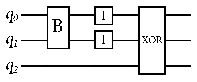
\includegraphics[width=0.3\textwidth]{images/testpathgadget.pdf}
\end{subfigure}
\begin{subfigure}
   \centering
   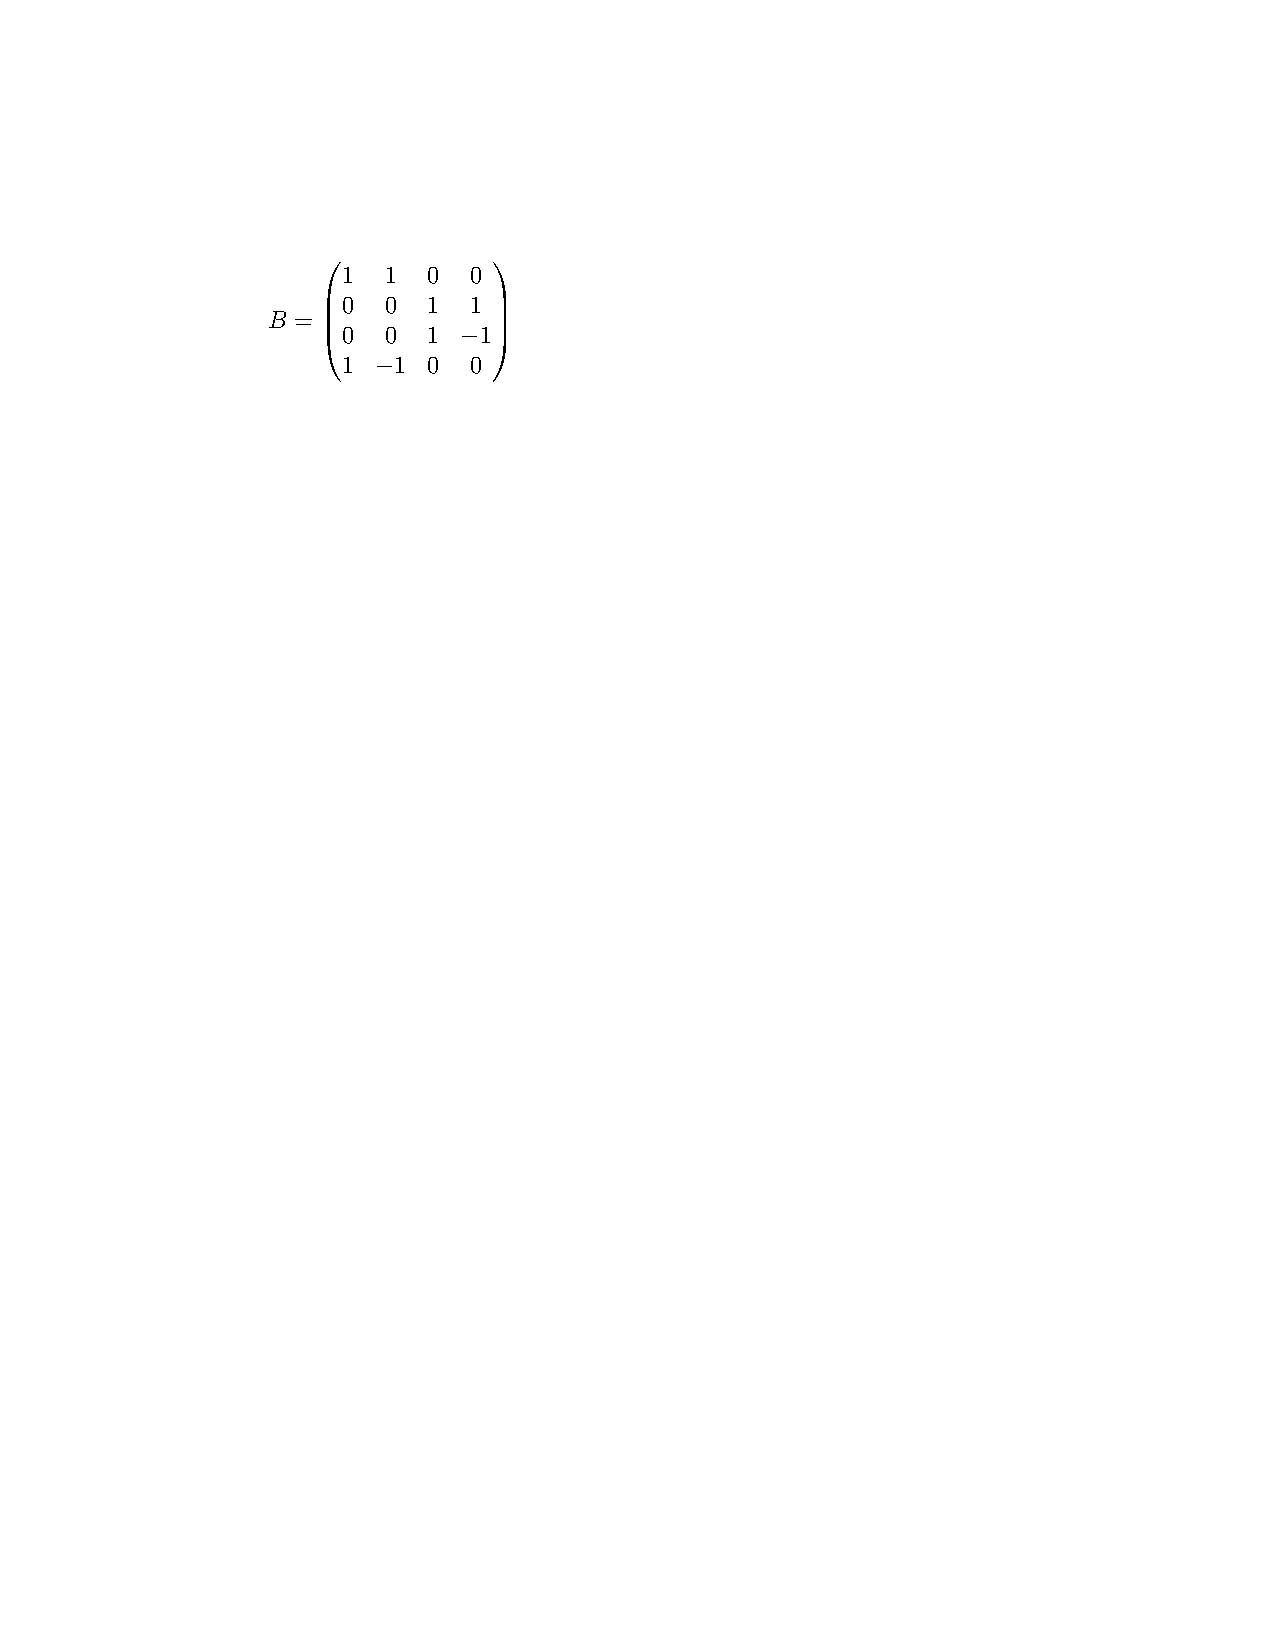
\includegraphics[width=0.25\textwidth]{images/bmatrix.pdf}
\end{subfigure}
\caption{Left: the circuit for Lemma~\ref{lem:testpath}. Right: the columns of
$B$ form the Bell basis.}
\label{fig:testpath}
\vskip -.26in
\end{figure}

\begin{small}
\bibliography{paper}
\end{small}

\end{document}
